\documentclass{beamer}

\usepackage{amsmath}
\usepackage{graphicx}
\usepackage{euler}
\usepackage{verbatim}

%Custom macros go here.

\newcommand{\Ei}{\textrm{Ei}} % Exponential integral
\newcommand{\Eig}{\textrm{Eig}} % Eigenvalues
\newcommand{\e}[0]{\hat{e}} % Unit vector
\newcommand{\norm}[1]{\left|\left|{#1}\right|\right|} % |n|
\newcommand{\fracflat}[2]{\left.{#1}\middle/{#2}\right.} % flat fractions
\newcommand{\flatfrac}[2]{\left.{#1}\middle/{#2}\right.} % flat fractions


\title{The Measurement of Anisotropic Thermal Conductivity in Snow With Needle Probes}
\subtitle{A Thesis Defense}
\author{Joshua Holbrook}
\date{April 4th, 2011}

\begin{document}
\frame{\titlepage}


\begin{frame}
\frametitle{Why Do We Study Snow's Thermal Conductivity?}
\begin{columns}[c]
\column{0.5\textwidth}
     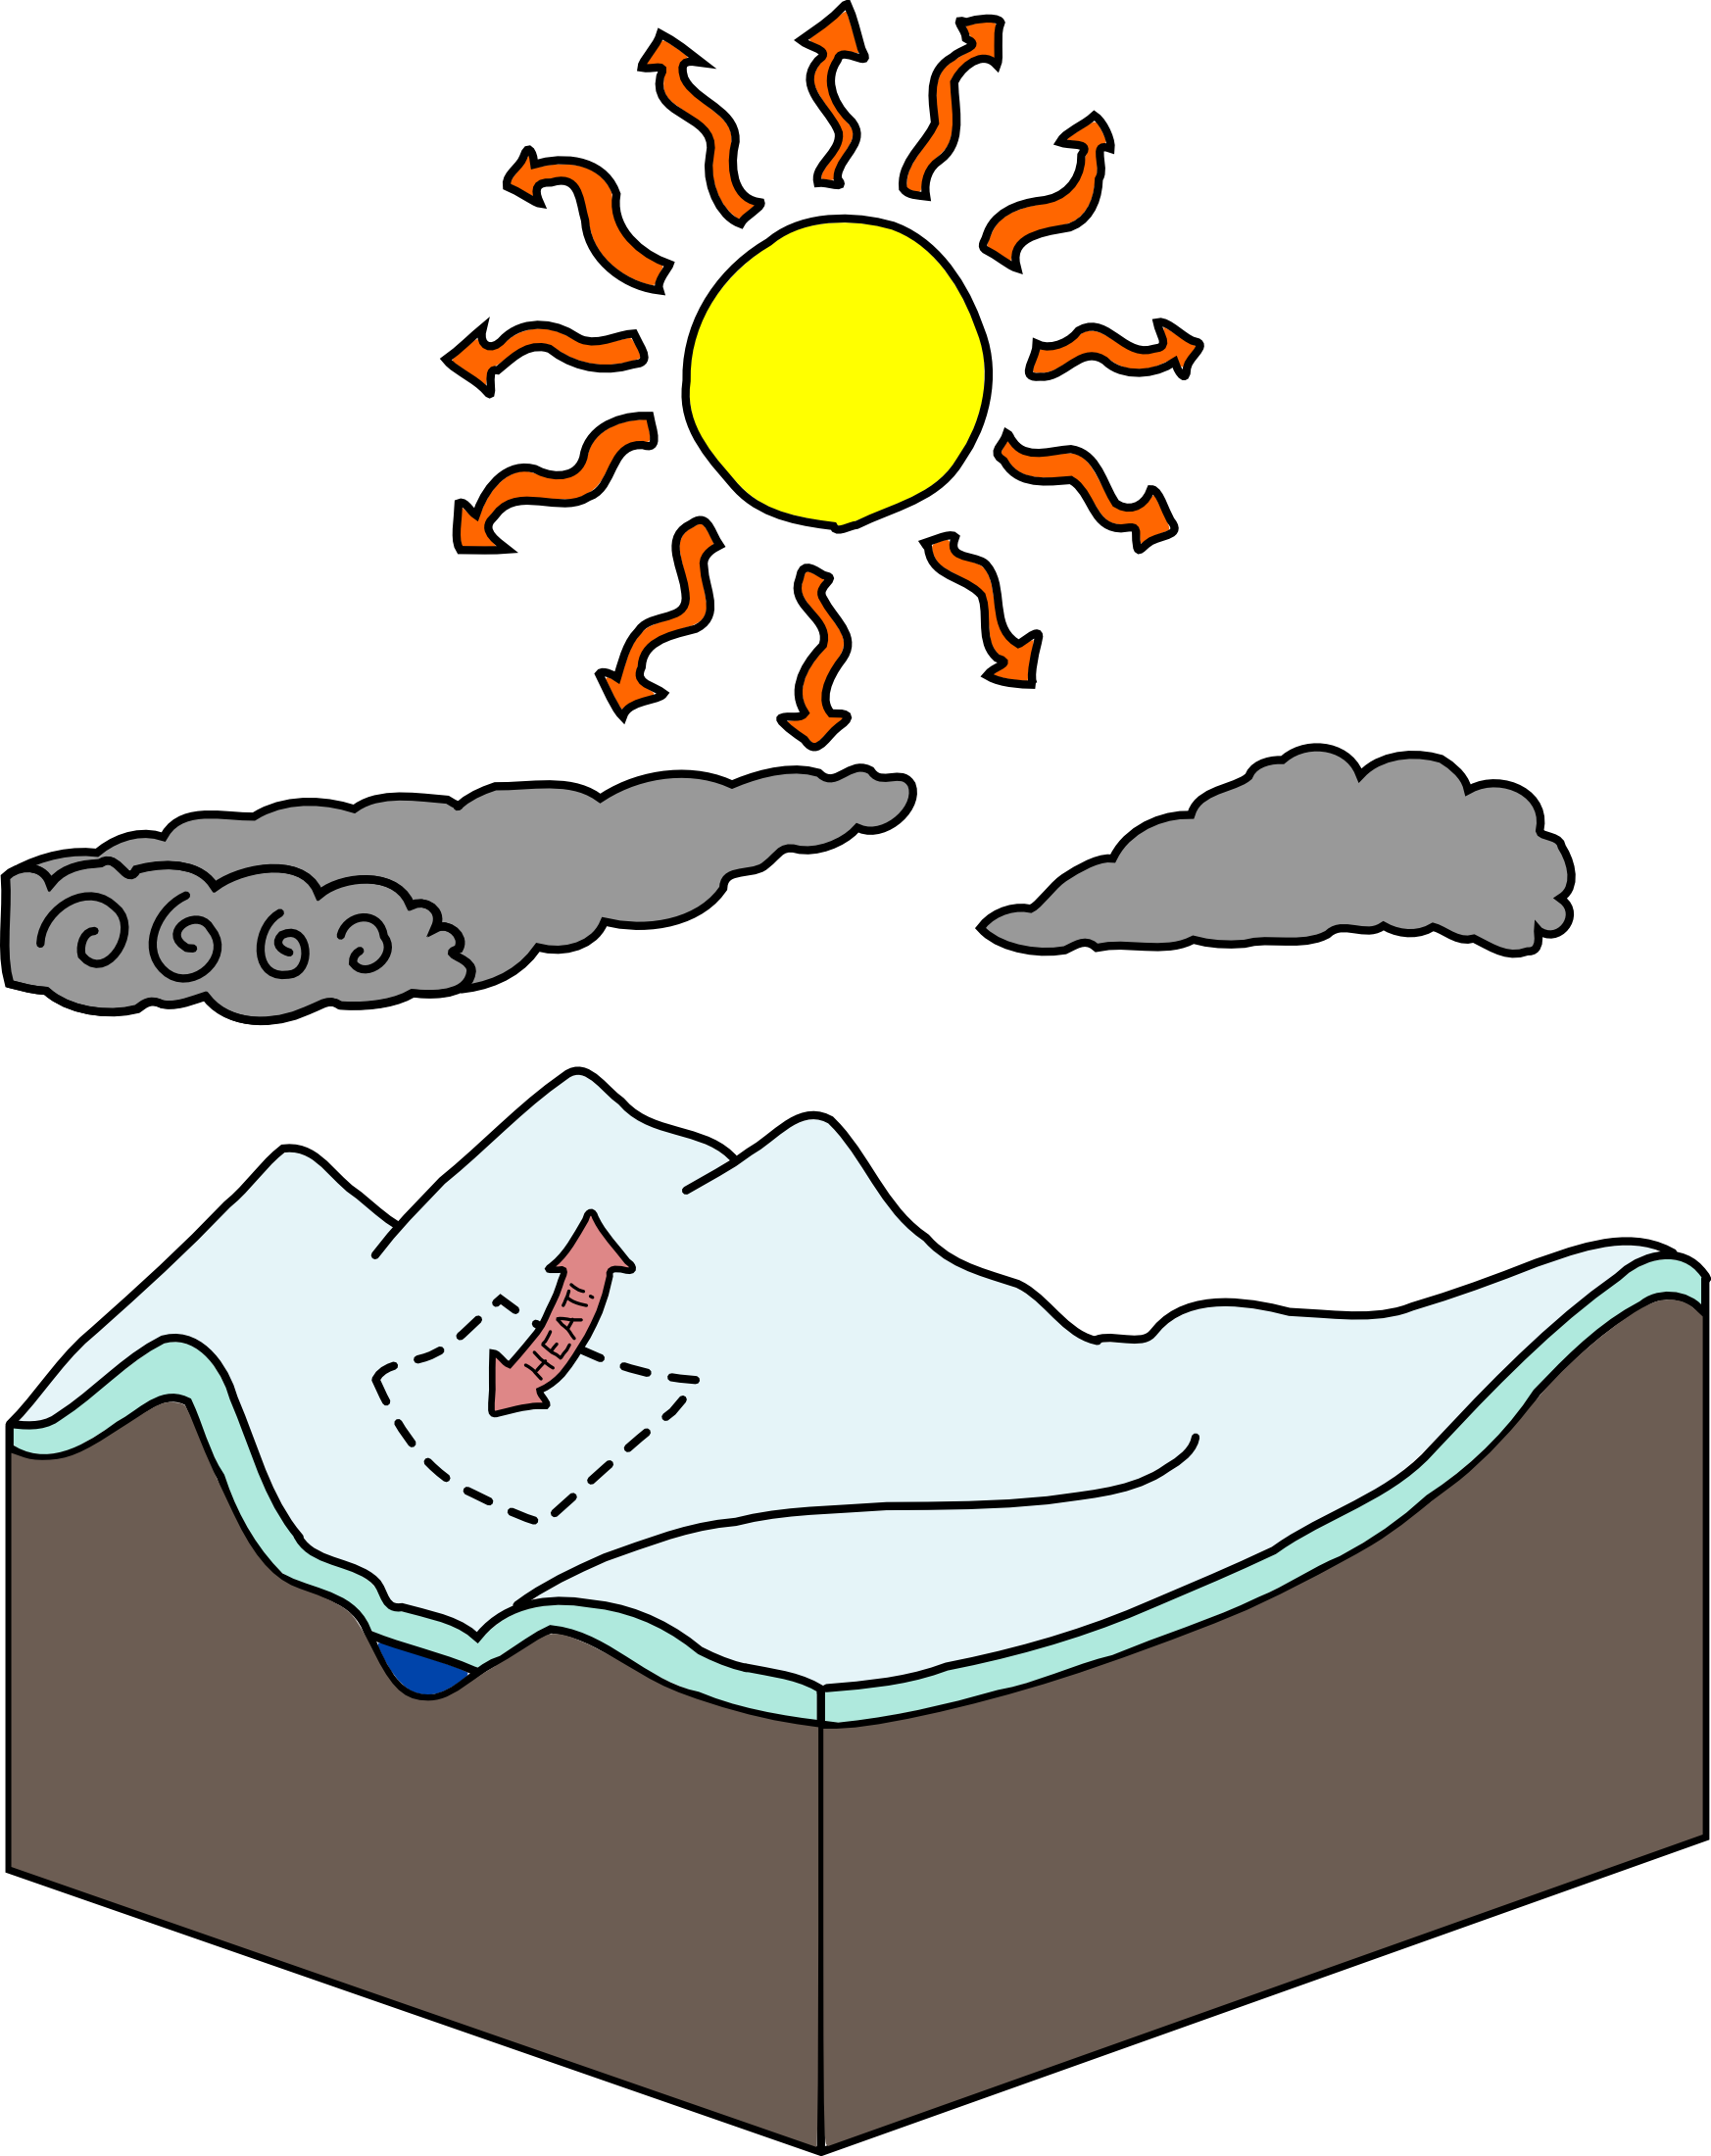
\includegraphics[width=\textwidth]{fig/climate.png}
\column{0.5\textwidth}
    \begin{itemize}
    \item Climatologists want to model Arctic climates.
    \item Heat transfer occurs between the earth and the atmosphere.
    \item Snow gets in the way. It's an \emph{insulating blanket}.
    \end{itemize}
\end{columns}
\end{frame}


\begin{frame}
\frametitle{How Do We Measure Thermal Conductivity?}
    \begin{itemize}
    \item One way is a guarded hot plate.
    \item Steady state 1-D conduction: \(k = \frac{\dot{q}l}{A\Delta T}\)
    \item Guarded hot plates are good for measuring foam boards.
    \item Guarded hot plates aren't exactly ideal for snow.
    \end{itemize}
\end{frame}


\begin{frame}
\frametitle{There HAS to be a better way.}
\begin{columns}[c]
\column{0.5\textwidth}
     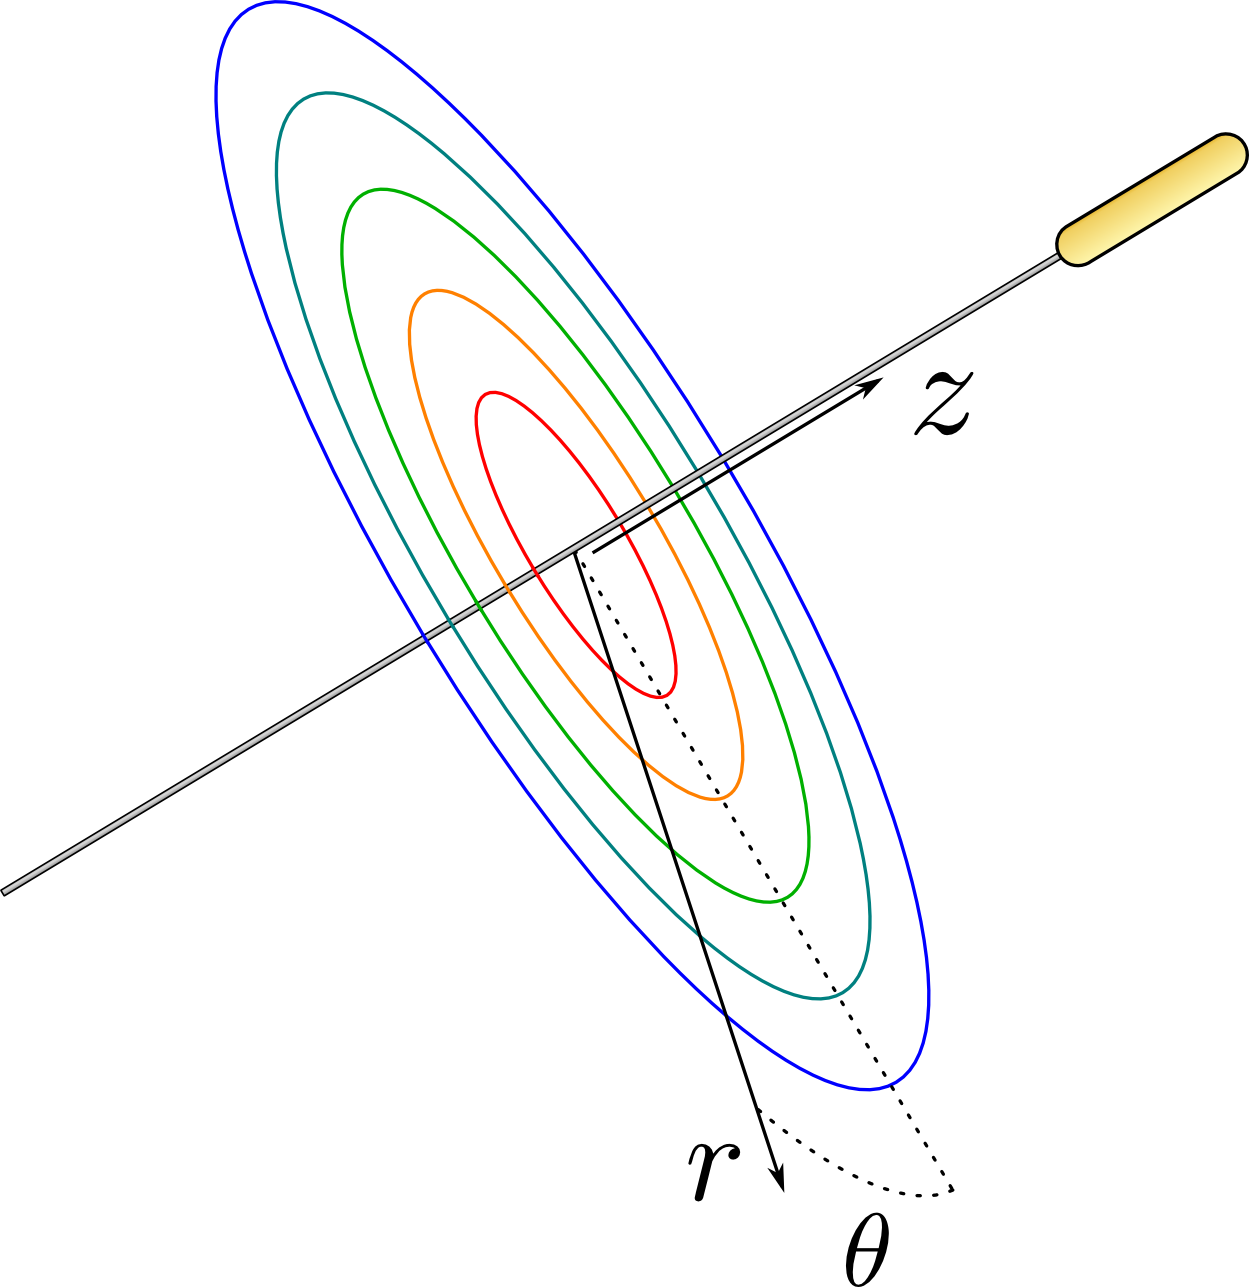
\includegraphics[width=\textwidth]{fig/basic_geometry.png}
\column{0.5\textwidth}
    \begin{itemize}
    \item It's called a needle probe.
    \item It looks something like this.
    \item It does \emph{not} use steady-state conduction.
    \item It depends on a \emph{radial} geometry.
    \item Okay, I'll admit, ``better'' is relative here.
    \end{itemize}
\end{columns}
\end{frame}


\begin{frame}
\frametitle{What Is A Needle Probe, Exactly?}
\begin{columns}[c]
\column{0.5\textwidth}
    \begin{itemize}
    \item Long and thin enough to approximate a line.
    \item Has a thermocouple in the center.
    \item Has heat trace running down most of its length.
    \item This is a drawing of a cross-section of such a needle (The one
          actually used has a slightly different configuration).
    \end{itemize}
\column{0.5\textwidth}
     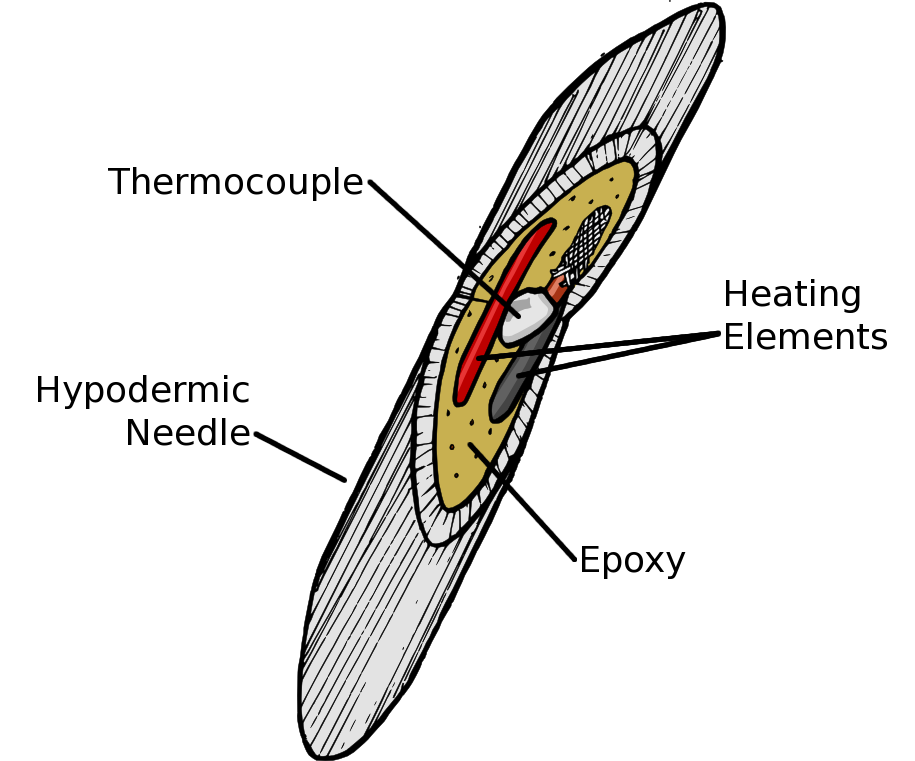
\includegraphics[width=0.8\textwidth]{fig/needle_xsect.png}
\end{columns}
\end{frame}


\begin{frame}
\frametitle{How Do You Measure \emph{Isotropic} Thermal Conductivity With It?}

\begin{columns}[c]
\column{0.3\textwidth}
    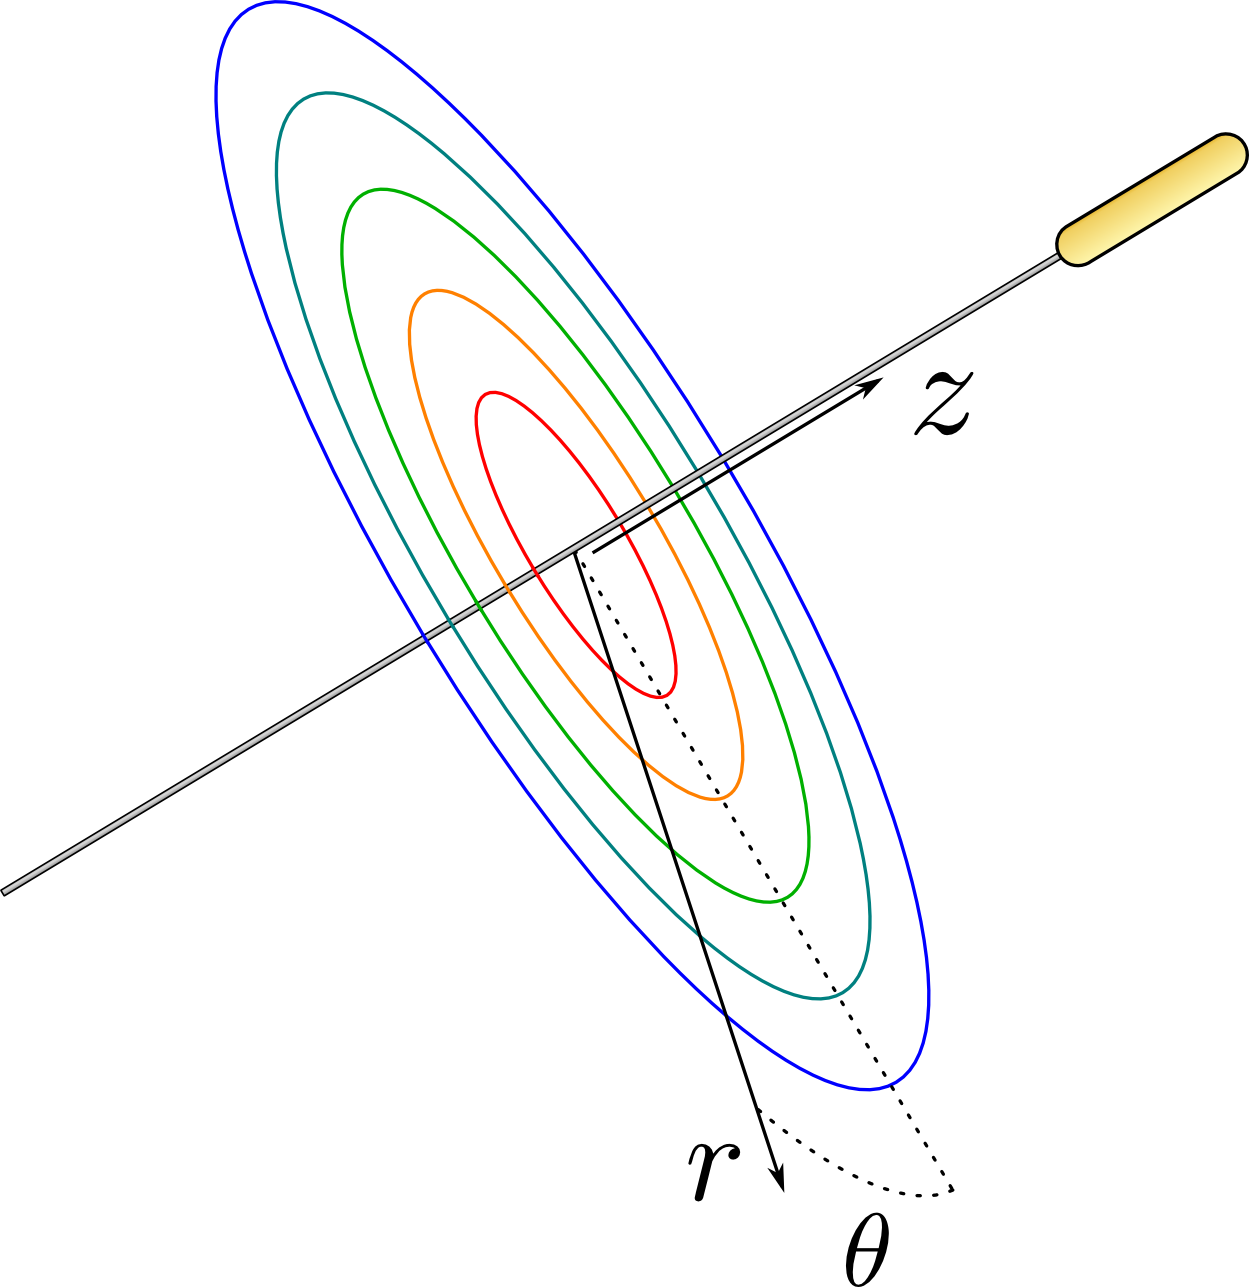
\includegraphics[width=\textwidth]{fig/basic_geometry.png}
\column{0.7\textwidth}
    \begin{enumerate}
    \item Write down The Heat Equation (\( -k\nabla^2 T = \rho C\frac{\partial T}{\partial t} \) in 3D Cartesian coordinates---Note the constant \(k\)
    simplification).
    \item Pose your problem in cylindrical coordinates, with constant heat flux at \(z=0\)
    \item Find a book where somebody has solved it for you already
    (Carslaw \& Jaeger) and write down the solution:

    \begin{equation*}
    T(r,t) = -\frac{q}{4\pi k}\Ei\left(-\frac{r^2}{4kt}\right)
    \end{equation*}

    \end{enumerate}
\end{columns}
\end{frame}


\begin{frame}
\frametitle{\(\Ei()\)? What's \emph{that}?}

\[\Ei(x) = -\int_{-x}^{\infty} \frac{e^{-t}}{t}dt \]

\begin{itemize}
\item ...in \emph{this} case. Some people define it differently.
\item You can't do that integral analytically, unfortunately.
\item \emph{However}, there \emph{are} long-time, small-radius approximations.
Hooray!
\end{itemize}
\end{frame}


\begin{frame}
\frametitle{Useful Approximation Action}

Over time, the solution approaches this:

\begin{equation*}
T(r,t) = \frac{q}{4\pi k}\ln\left(\frac{4kt}{r^2}\right) - \frac{\gamma q}{4\pi k}
\end{equation*}

But, more usefully:

\begin{equation*}
\frac{\partial T}{\partial \ln(t)} = \frac{q}{4\pi k}
\end{equation*}

\end{frame}


\begin{frame}
\frametitle{Finding Conductivities: A Real-Life Example}

This is a temperature/time curve for an actual measurement of snow behind my
house:

\begin{columns}[c]
\column{0.6\textwidth}
    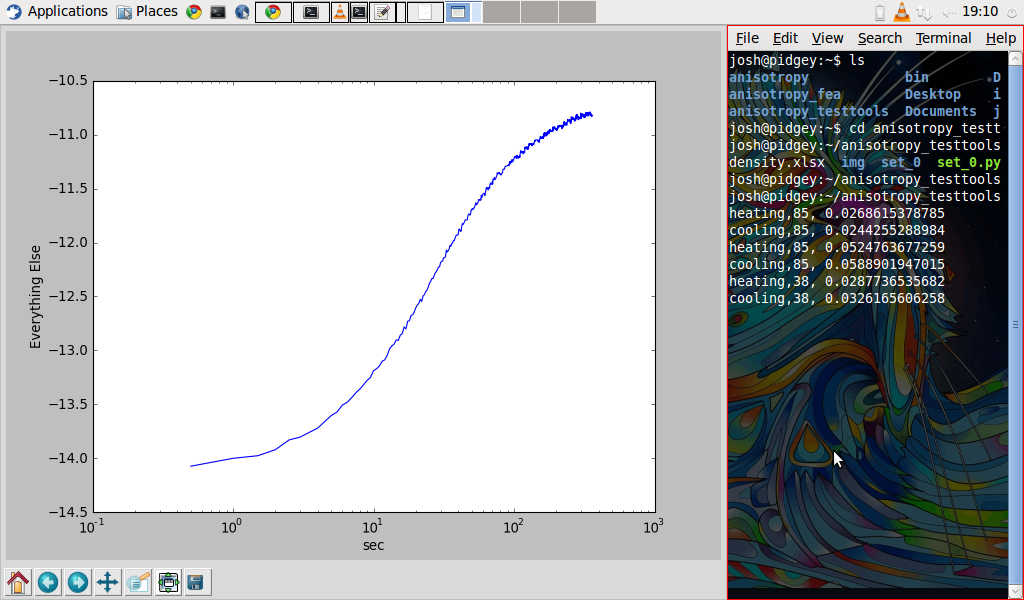
\includegraphics[width=\textwidth]{fig/measurement_graph.png}
\column{0.4\textwidth}
    \begin{itemize}
    \item Early ``transient'' behavior (The whole situation's transient conduction)
    \item Mid-range, steady-slope behavior (This is what we're interested in)
    \item Late-game in-snow convection (Can be mitigated by using less heat)
    \end{itemize}
\end{columns}
\end{frame}


\begin{frame}
\frametitle{There's a Cooling Curve, As Well}
\begin{itemize}
\item That was what's called the ``heating curve.''
\item The ``cooling curve'' is when you watch the needle cool back down.
\item By an analogous derivation, we can find a similar long-time solution for
cooling curve slope over \(\ln(t_{\textrm{cooling}})\)
\item Used in measurements, but not modeled. Sorry, guys.
\end{itemize}
\end{frame}


\begin{frame}
\frametitle{Metamorphic Powder Rangers: How Snow Becomes Anisotropic}
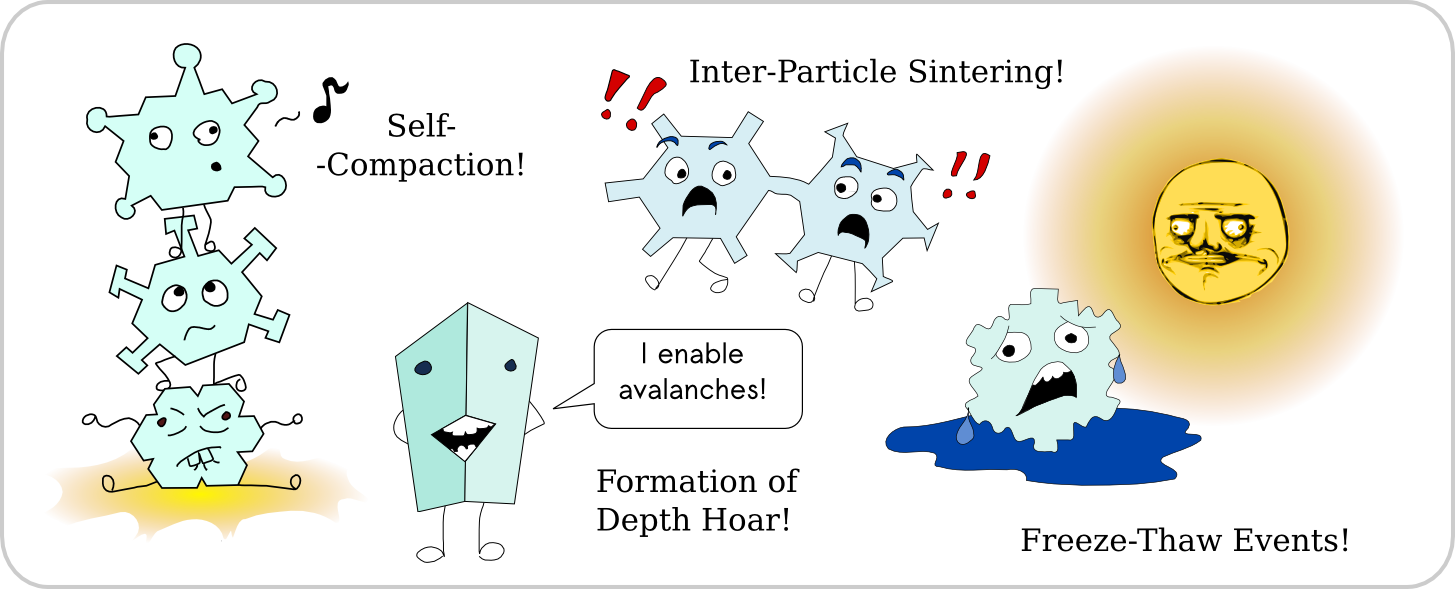
\includegraphics[width=\textwidth]{fig/metamorphism.png}\\
These processes cause snow to form regions of varying thermal conductivity---for
example, alternating layers of high and low conductivity.
\end{frame}


\begin{frame}
\frametitle{Example Time!}
\begin{columns}[c]
\column{0.5\textwidth}
    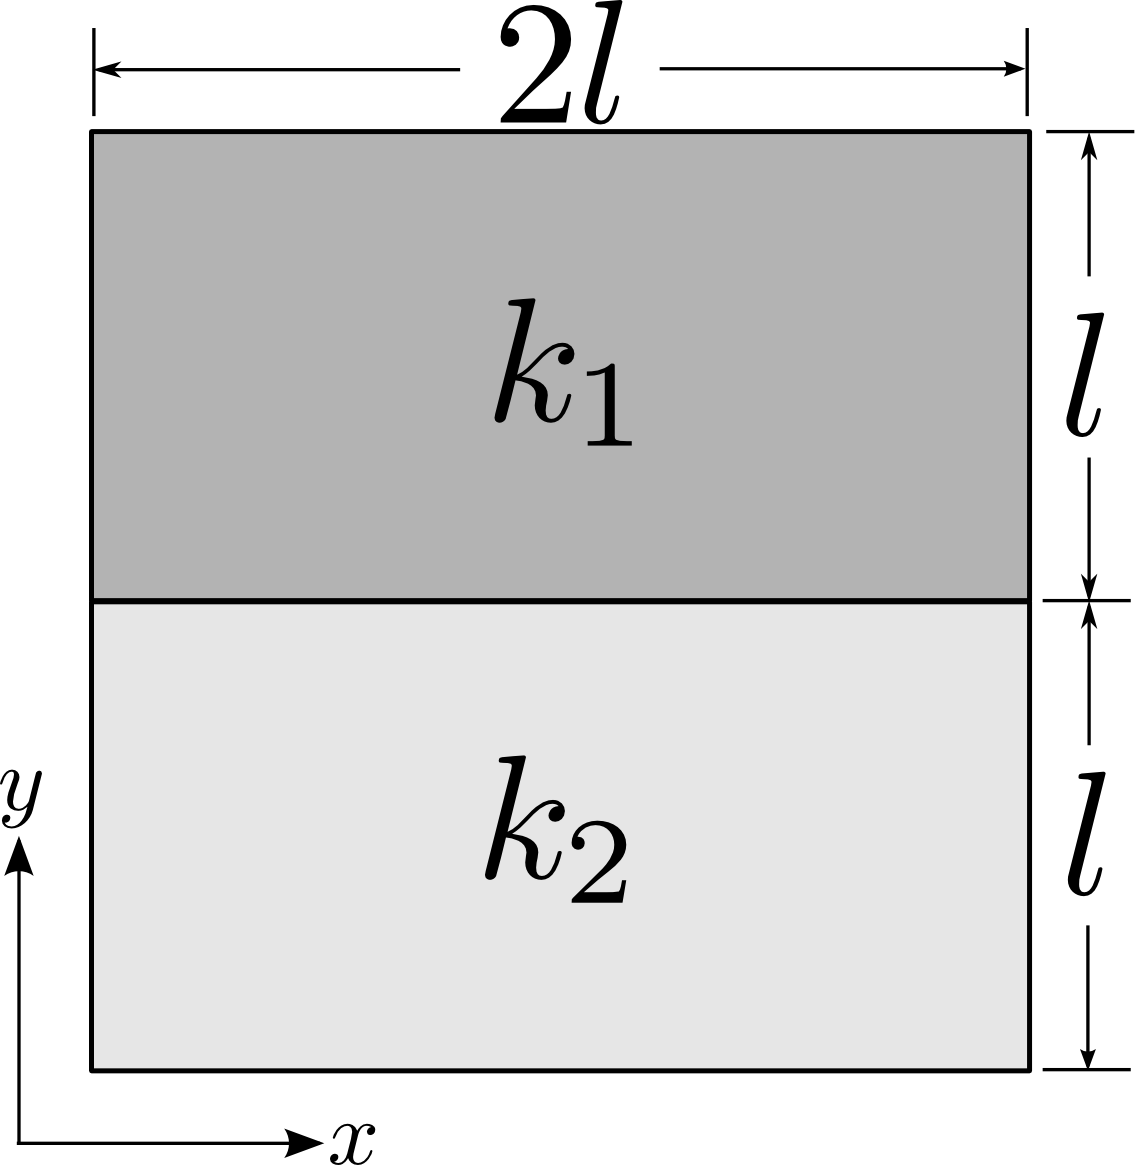
\includegraphics[width=0.7\textwidth]{fig/ex_laminate.png}
\column{0.5\textwidth}
    \begin{itemize}
    \item Vertically: \(\frac12(k_1 + k_2)\)
    \item Horizontally: \(2\left( \frac1{k_1} + \frac1{k_2} \right)^{-1}\)
    \end{itemize}
\end{columns}
\smallskip
Keep this example in mind for later!
\end{frame}

\begin{comment}
Note: We can also discuss some of the questions being brought up, but I'd like
to Broad Overview this.
\end{comment}

\begin{frame}
\frametitle{The Basic Model}
\begin{columns}[c]
\column{0.4\textwidth}
    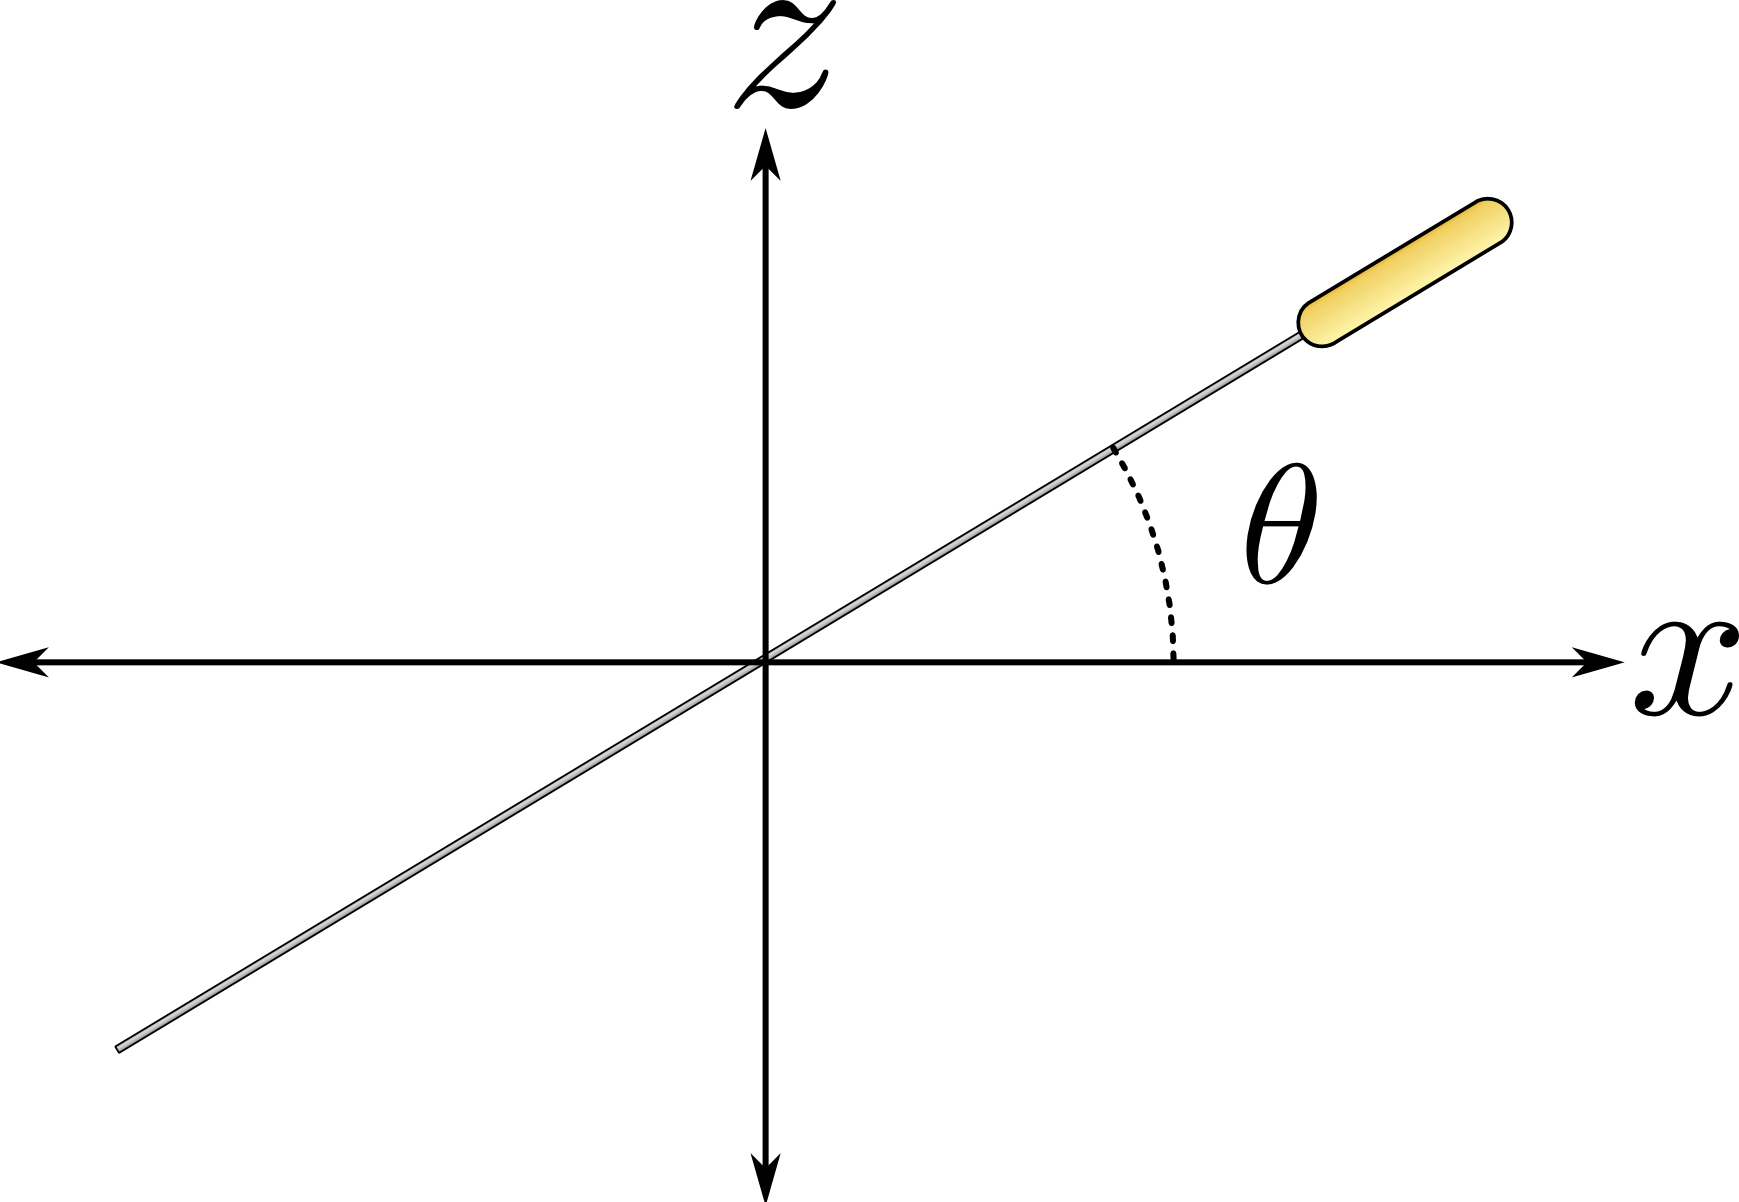
\includegraphics[width=\textwidth]{fig/angle.png}
\column{0.6\textwidth}
    \begin{itemize}
    \item Horizontal and Vertical conductivities only.
    \item Needle rotated from the horizontal.
    \item Goal: Find \(k_{\textrm{meas}}(\theta)\) for a given \(k_{xy}\) and \(k_z\).
    \end{itemize}
\end{columns}
\end{frame}


\begin{frame}
\frametitle{Outline!}
\begin{itemize}
\item Analytical Approaches
\item Numerical Modeling in COMSOL
\item Measurements of Snow and Engineered Materials
\item Results
\item Loose Ends
\end{itemize}
\end{frame}


\begin{frame}
\frametitle{Analytical Approaches}
\begin{columns}[c]
\column{0.5\textwidth}
    \begin{itemize}
    \item We already have a working isotropic theory
    \item But for the anisotropic case, the conductivity is a \(3\times 3\), positive definite matrix!
    \item Can we adapt the isotropic theory to the anisotropic cases? (Yes.)
    \end{itemize}
\column{0.5\textwidth}
    \begin{equation*}
    \nabla\begin{bmatrix}
    k_{11} & k_{12} & k_{13}\\
    k_{12} & k_{22} & k_{23}\\
    k_{13} & k_{23} & k_{33}
    \end{bmatrix}\nabla T = -\rho C\frac{\partial T}{\partial t}
    \end{equation*}
\end{columns}
\end{frame}


\begin{frame}
%That texttt mess is for making the dashes not blend.
\frametitle{First: \texttt{dimension-}\texttt{-;}}
\centering
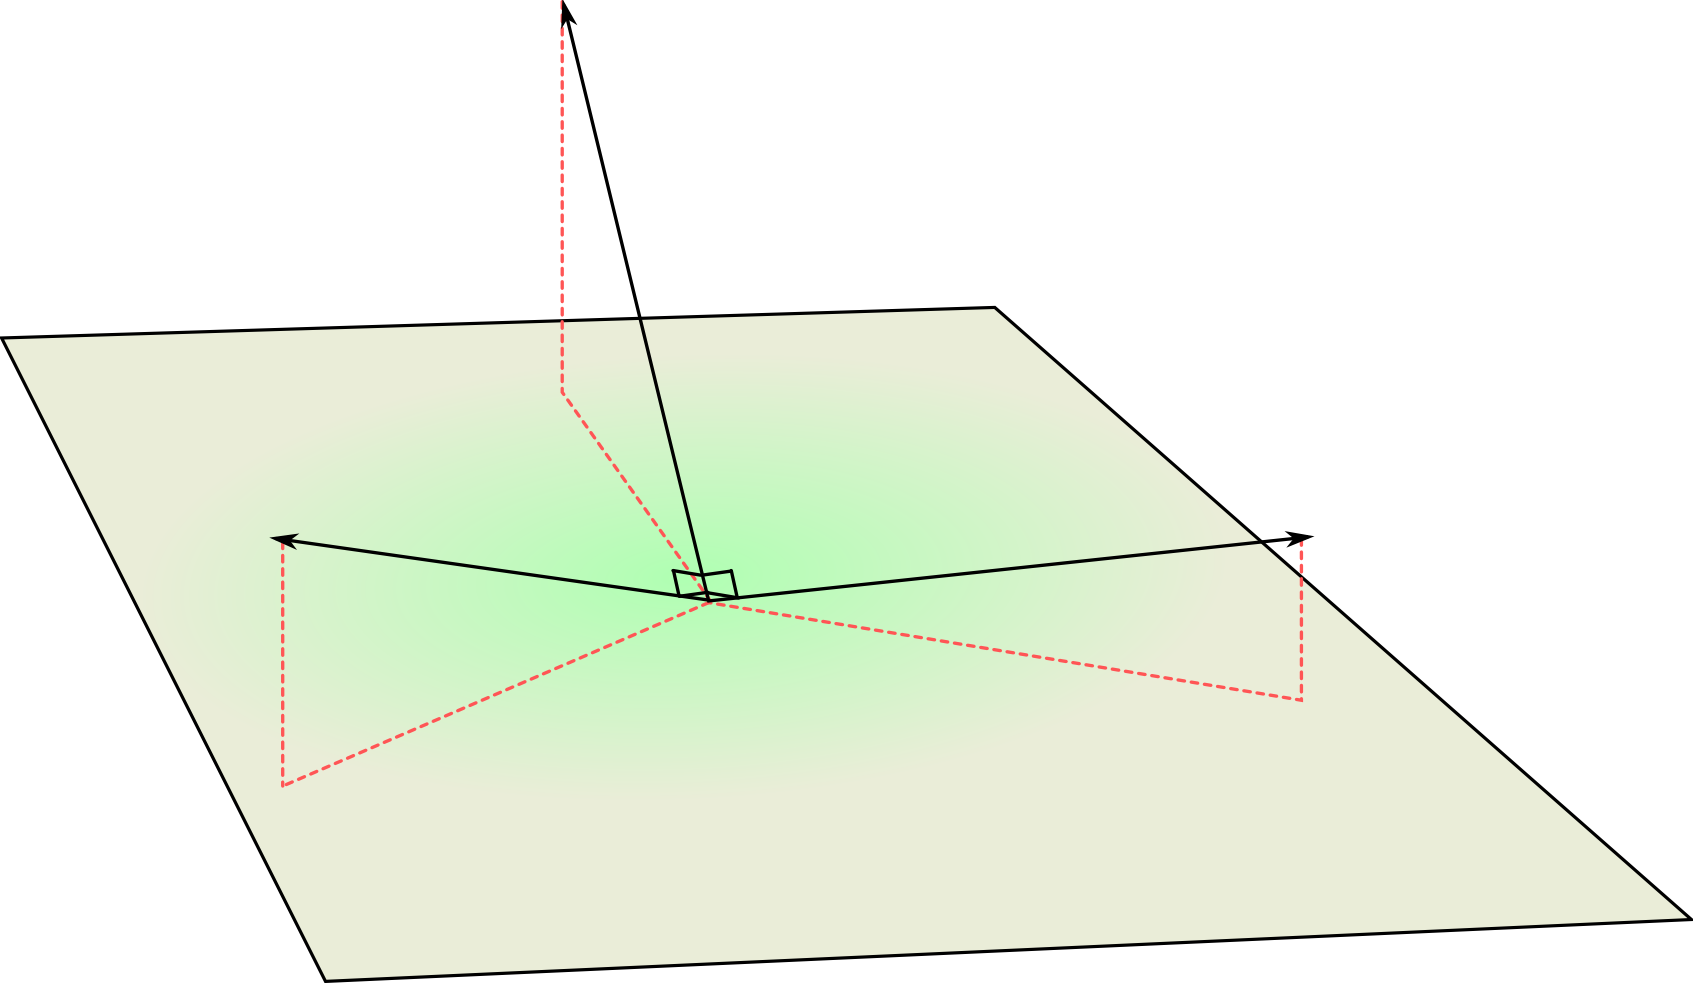
\includegraphics[width=0.6\textwidth]{fig/projection.png}
\begin{itemize}
\item Remember, there's no temperature gradient in the \(z\) direction!
\item First, drop the \(z\) coordinates, then find the positive eigenvalues.
\end{itemize}
\end{frame}

\begin{frame}
\frametitle{Second: Stretch!}
We now have:
\begin{equation*}
-\nabla \cdot \left(\begin{bmatrix}k_x & 0\\ 0 & k_y\end{bmatrix}\nabla T \right)= \rho C\frac{\partial T}{\partial t}
\end{equation*}

\begin{columns}
\column{0.5\textwidth}
    \begin{itemize}
    \item What if we use a different coordinate system (\(x'\) and \(y'\)) to make
    that matrix a multiple of \([I]\)?
    \end{itemize}
\column{0.5\textwidth}
    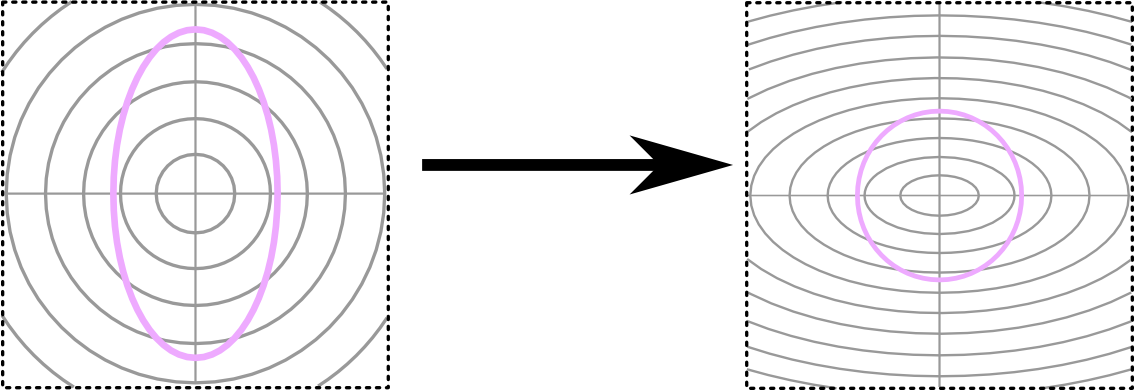
\includegraphics[width=\textwidth]{fig/coordinate_transformation.png}
\end{columns}
\end{frame}

\begin{frame}
\frametitle{Math Alert! Math Alert!}

\begin{align*}
x' &= a_x x\\
y' &= a_y y\\
a_x &= 1 \textrm{ (WLOG)}
\end{align*}
\begin{align*}
\frac{dx'}{dx} &= 1\\
\frac{dy'}{dy} &= a_y
\end{align*}
\end{frame}


\begin{frame}
\frametitle{It's Not Over Yet.}
\begin{align*}
\frac{\partial f}{\partial x} &= \frac{\partial f}{\partial x'}\frac{dx'}{dx} = \frac{\partial f}{\partial x'}\\
\frac{\partial f}{\partial y} &= \frac{\partial f}{\partial y'}\frac{dy'}{dy} = a_y\frac{\partial f}{\partial y'}
\end{align*}

\begin{align*}
\nabla T &= \frac{\partial T}{\partial x'} \e_{x'} + a_y\frac{\partial T}{\partial y'} \e_{y'} \\
[K]\nabla T &= k_x\frac{\partial T}{\partial x'} \e_{x'} + k_ya_y\frac{\partial T}{\partial y'} \e_{y'}\\
\nabla \cdot \left([K]\nabla T\right) &= k_x\frac{\partial^2 T}{\partial {x'}^2} + k_ya_y^2\frac{\partial^2 T}{\partial {y'}^2}\\
\end{align*}
\end{frame}


\begin{frame}
\frametitle{Almost Done!}
Suppose the right hand side is equal to the equivalent isotropic expression:
\begin{equation*}
k\left(\frac{\partial^2 T}{\partial {x'}^2} + \frac{\partial^2 T}{\partial {y'}^2} \right) = k_x\frac{\partial^2 T}{\partial {x'}^2} + k_ya_y^2\frac{\partial^2 T}{\partial {y'}^2}
\end{equation*}

THIS MEANS:

\begin{align*}
k &= k_x\\
a_y &= \sqrt{\frac{k_x}{k_y}}
\end{align*}
\end{frame}

\begin{frame}
\frametitle{But Then, A Shocking Twist.}
\begin{equation*}
T(r',t) = \frac{q}{4\pi k_x}\ln\left(\frac{4k_xt}{r'^2}\right) - \frac{\gamma q}{4\pi k_x}
\end{equation*}
\begin{itemize}
\item This equation is in terms of \(r'\), not \(r\)!
\item If you try to take your derivative here, it \emph{will not work like you want it to}.
\item We need to do something with the \(r'\) this time.
\end{itemize}
\end{frame}


\begin{frame}
\frametitle{What Is \(r\) \emph{Anyway?}}
\begin{itemize}
\item Arguably, our Actual Measurement is the average temperature at some finite 
\(r\) from the center of the needle.
\item There are other approaches one may take, such as assuming a non-zero needle
thickness in the problem formulation.
\item It can be shown (as it is in the thesis) that:
\begin{equation*}
    \norm{r'}^2 = r_0^2 \left(\cos^2(\theta) + \frac{k_x}{k_y}\sin^2(\theta) \right)
\end{equation*}
\item Note, \(r'\) is a function of \(\theta\).
\end{itemize}
\end{frame}


\begin{frame}
\frametitle{Elliptical Integral Time}
\begin{itemize}
\item Taking the averaging approach, our problem can now be described as so:
\begin{equation*}
T_{\textrm{avg}}(t) = \frac{4\pi k_x}{q} \frac{\mathcal{E}(\ln(t), \frac{k_y}{k_x})}{\mathcal{E}(1, \frac{k_y}{k_x})}
\end{equation*}

\item What's this \(\mathcal{E}\) stuff?
\begin{equation*}
\mathcal{E}(f(\phi, \alpha), \alpha) = \int_0^{2\pi} f\sqrt{\cos^2(\phi) + \alpha\sin^2(\phi)} d\phi
\end{equation*}
\item Curve fit \emph{this} equation to the \(T = A \ln(t) + C\) form, and you now
have a \(k_{\textrm{meas}}\)!
\end{itemize}
\end{frame}


\begin{frame}
\frametitle{Implementation Notes}
\begin{itemize}
\item I used python and numpy/scipy.
\item Integrals are evaluated numerically using a quadrature method.
\item Source available upon request.
\end{itemize}
\end{frame}


\end{document}


